\chapter{Théorie des Graphes}


\section{Chemins et connectivité}
Nous allons commencer par rappeler la notion de chemin:
	\begin{description}
	\item[Chemin]: c'est une séquence de n\oe uds dont chaque paire consécutive est une arrête.
    \item[Chemin simple]: c'est un chemin dont chaque n\oe ud se trouve au maximum une fois dans la séquence de n\oe uds.
    \item[Cycle]: c'est un chemin dont le premier et le dernier n\oe ud sont le même. Un cycle possède au moins 3 liens (arrêtes).\\
	\end{description}

Maintenant, nous allons définir la notion de connectivité d'un graphe.
	\begin{description}
    \item[Connectivité]: un graphe est dit connexe si pour toutes paires de n\oe uds A et B, il existe au moins un chemin de A vers B.\\
	\end{description}

Tous les graphes ne sont en effet pas connexe. La figure \ref{graphe_non_connexe} montre un exemple de graphe non connexe.
	\begin{figure}
	\center
	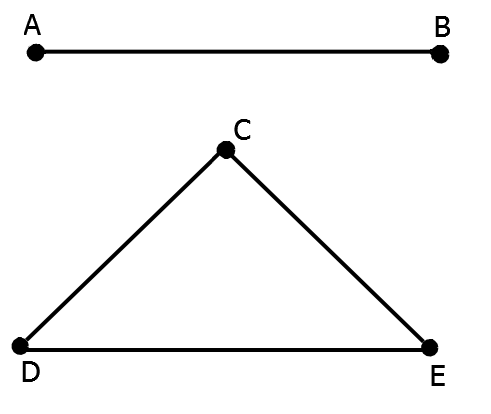
\includegraphics[scale=0.3]{images/18_graphe_non_connexe.png}
	\caption{\label{graphe_non_connexe} Graphe non connexe}
	\end{figure}
Ce graphe possède deux composants, $AB$ et $CDE$. Ces composants (qui sont maximals) sont les parties connexes du graphe. On a les définitions suivantes:
	\begin{description}
    \item[Composant d'un graphe]: c'est un sous-graphe (partie de graphe) qui est connexe. Il est maximal s'il ne fait pas partie d'un composant plus grand.
    \item[Composant géant] : il s'agit d'un composant qui contient une fraction significative de l'ensemble des n\oe uds contenus dans le graphe.
    \end{description}
    
    Par exemple, le graphe des amitiés mondiales n'est surement pas connexe. En effet, il peut y avoir des habitants d'une île reculée qui se connaissent entre eux, mais qui n'ont pas de connection avec le reste du monde. Cependant, la majorité du monde est connecté; on a donc un énorme composant géant.\\
    
    C'est une propriété générale des grands graphes complexes: il est rare qu'ils soient connexe, mais ils ont très souvent un composant géant. Avoir plusieurs composants géants est instable: il arrive vite qu'un lien se forme entre les deux composants, formant ainsi un seul composant géant. Si avant le \textsc{xv}\textsuperscript{ème} siècle il y avait un composant géant eurasien et un autre américain, il n'a fallu qu'un lien (la découverte de l'Amérique par Christophe Colomb) pour assembler les deux composants, avec toutes les conséquences que cela a entrainé (maladies, exploitation, etc.).\\
    
Avec les éléments que nous venons de définir, on est en mesure d'analyser tout un graphe. On peut le partitionner en composants et regarder la structure interne de chacun d'entre eux. Par exemple, dans la figure \ref{gr_connexe}, on peut partitionner en deux composantes, $ABC$ et $DEF$. On constate que le lien $CD$ est un lien spécial car si on l'enlève, il déconnecte de graphe.\\
	\begin{figure}
	\center
	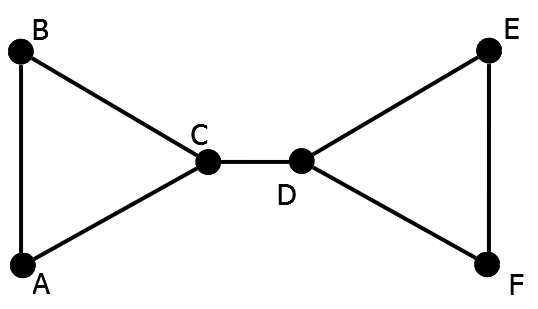
\includegraphics[scale=0.3]{images/18_gr_connexe.png}
	\caption{\label{gr_connexe} Graphe connexe}
	\end{figure}

\section{Distance entre n\oe uds}
Nous allons maintenant définir la longueur d'un chemin ainsi que la distance entre deux n\oe uds :
\begin{description}
\item[Longueur d'un chemin] : le nombre d'arêtes consécutives sur ce chemin.
\item [Distance entre 2 n\oe uds] : le chemin le plus court entre ces deux n\oe uds.
\end{description}

La méthode de calcul de distance entre deux n\oe ud est la traversée en largeur d'abord (\emph{breadth-first traversal}). Cela consiste à débuter par un n\oe ud, puis à regarder tous les n\oe uds qui sont à une distance de 1 du n\oe ud de départ. À partir de tous ceux-là, on regarder les n\oe uds qui sont à une distance 1, et donc à une distance 2 du n\oe ud de départ. On continue jusqu'à arriver au n\oe ud d'arrivée. On a donc à chaque étape constitué des couches de n\oe uds se trouvant à une certaine distance. Cet algorithme sera expliqué plus en détail par après.\\

\section{Phénomène du petit monde}
Le « phénomène du petit monde » aussi connu sous le vocable « paradoxe de Milgram » (du nom du psycho-sociologue Stanley Milgram) est l'hypothèse que chacun puisse être relié à n'importe quel autre individu par une courte chaîne de relations sociales. La figure \ref{petit_monde} montre la probabilité qu'ont deux personnes d'être relié par $x$ intermédiaires. 
	\begin{figure}
	\center
	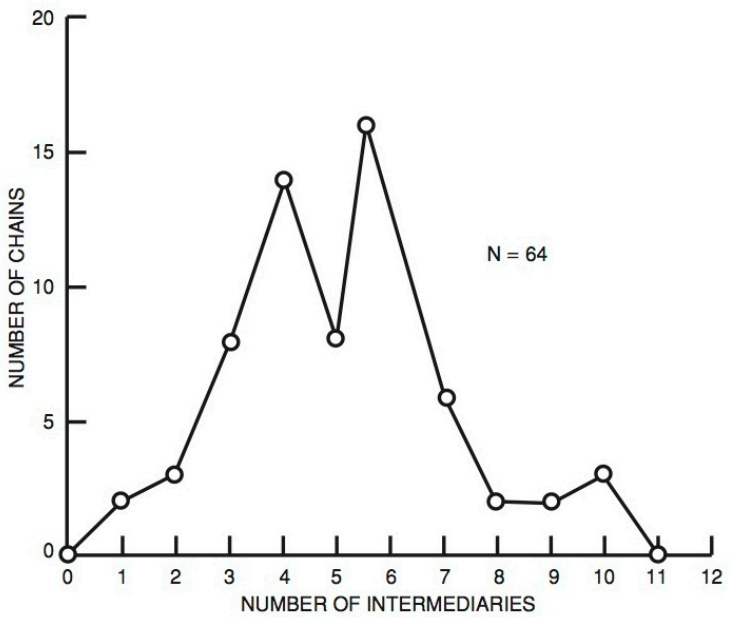
\includegraphics[scale=1]{images/18_fig.png}
	\caption{\label{petit_monde} Statistiques du phénomène du petit monde}
	\end{figure}
Cette  courte chaîne de relations sociales a été approfondie par la théorie des « six degrés de séparation » affirmant qu'en prenant deux personnes, il est possible de trouver une chaîne d'amis entre eux de taille maximum 6.
Différents types de distances entre personnes existent comme:
	\begin{itemize}
	\item Le nombre d'Erdos est la distance de collaboration avec le célèbre mathématicien Paul Erdös qui a réalisé de très nombreuses co-publications. Avoir réalisé une publication en collaboration avec Erdös correspond au nombre d'Erdös 1. Avoir écrit une publication avec quelqu'un qui a co-publié avec Erdös équivaut au nombre 2, etc.
	\item Le nombre de Bacon est la distance de collaboration dans un film avec l'acteur Kevin Bacon.
	\end{itemize}
Ce phénomène de petit monde est particulièrement vrai pour les réseaux créés dynamiquement. Nous expliquerons plus en détail pourquoi cette affirmation est vraie dans la suite du cours.

\section{Liens forts et faibles}
Un réseau peut évoluer de différentes manières et selon différents mécanismes.
Considérons un exemple ou chaque n\oe ud correspond à une personne et les arcs correspondent à un lien d'amitié (figure \ref{fermeture_triadique}).
	\begin{figure}
	\center
	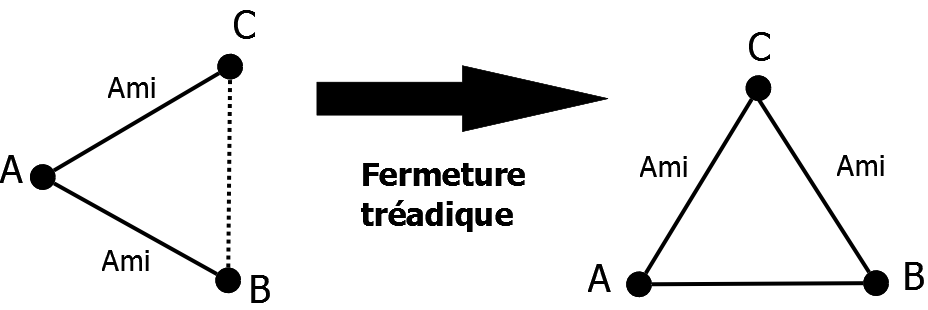
\includegraphics[scale=0.5]{images/18_fermeture_triadique.png}
	\caption{\label{fermeture_triadique} Exemple de fermeture triadique}
	\end{figure}
Dans cet exemple, on voit aue $A$ est amis à la fois avec $B$ et avec $C$. Dans cette condition, il est port probable que $B$ et $C$ deviennent eux-mêmes amis. C'est ce qu'on appelle la fermeture triadique.\\
\\
Cette situation nous amène à nous intéresser à la notion de coéficient de regroupement qui reflète la probabilité qu'un arc se crée entre deux n\oe uds dans un graphe dynamique. 
Dans l'exemple ci-dessus, cela correspondrait au fait que C et B deviennent amis. On peut démontrer qu'au plus on fait de fermeture triadique, au plus le coeficient de regroupement est elevé.

\subsection*{Exemple}
Une étude a été faite dans les années 1960 par le sociologue américain Mark Granovetter dans laquelle il s'est interessé aux personnes qui changent de travail, plus particulièrement à la manière dont ils trouvent un nouveau travail. Il a remarqué que les personnes trouvent du travail plutôt via des connaissances que via des amis. Cela s'explique par la structure des graphe des amis et nous amène à définir les notions de \textbf{liens forts} et de \textbf{liens faibles} (figure \ref{liens_forts_et_faibles}). La suite de cet exemple sera expliqué plus tard.\\
	\begin{figure}[!h]
	\center
	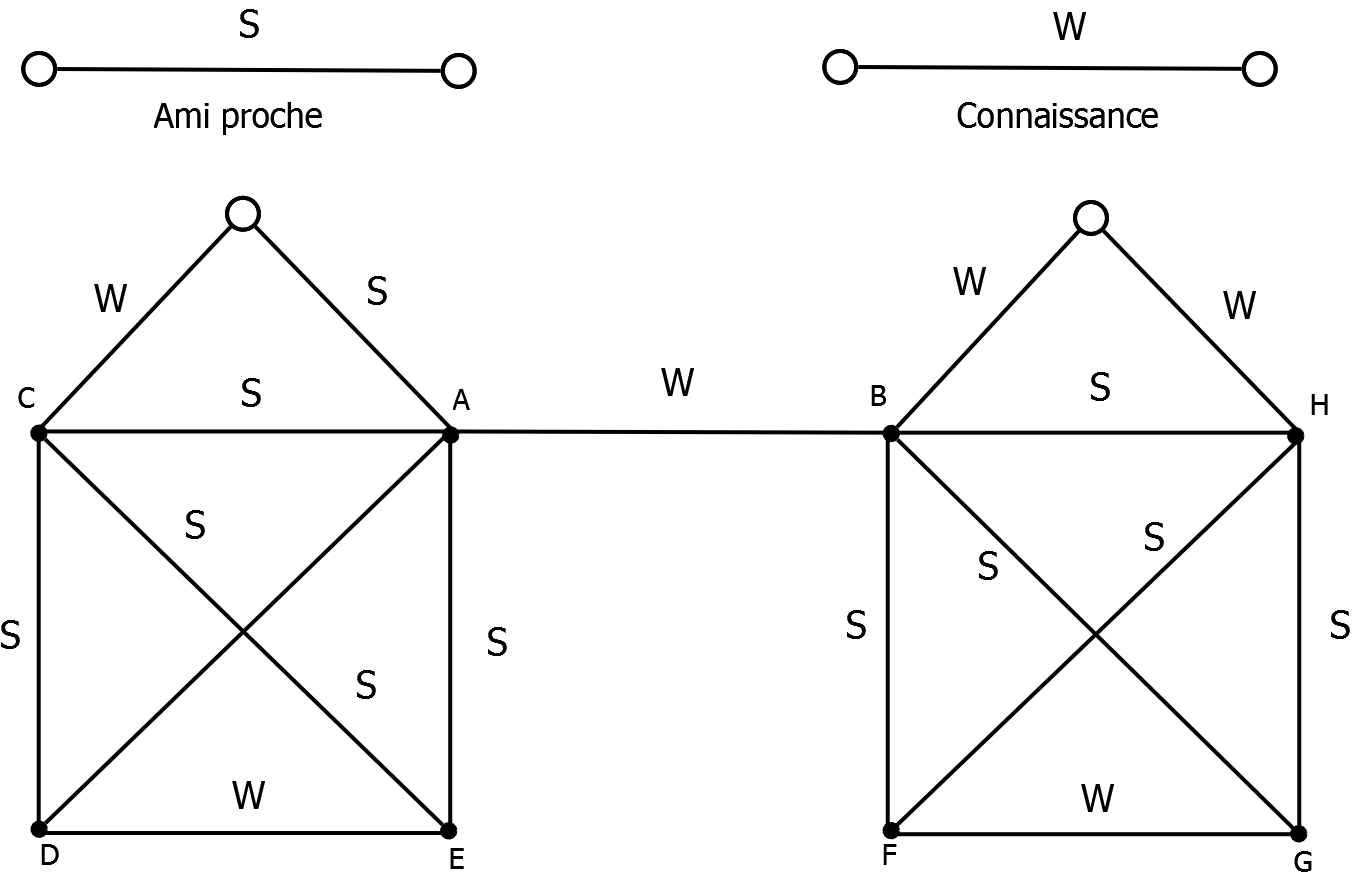
\includegraphics[scale=0.4]{images/18_liens_forts_et_faibles.png}
	\caption{\label{liens_forts_et_faibles} Liens forts et faibles}
	\end{figure}

    
\section{Ponts}
Pour expliquer l'exemple précédent, nous avons besoin de la notion de pont (figures \ref{Pont} et \ref{Pontlocal}).
	\begin{description}
	\item[Pont] Un lien entre $A$ et $B$ est un pont si l'enlèvement de ce lien aboutit à la séparation du graphe en deux composants disjoints.
    \item[Pont local] Un lien entre $A$ et $B$ est un pont local si l'enlèvement de ce lien aboutit au fait que deux composantes sont reliées par un chemin significativement plus long.
    \end{description}
    
    \begin{figure}
    \center
    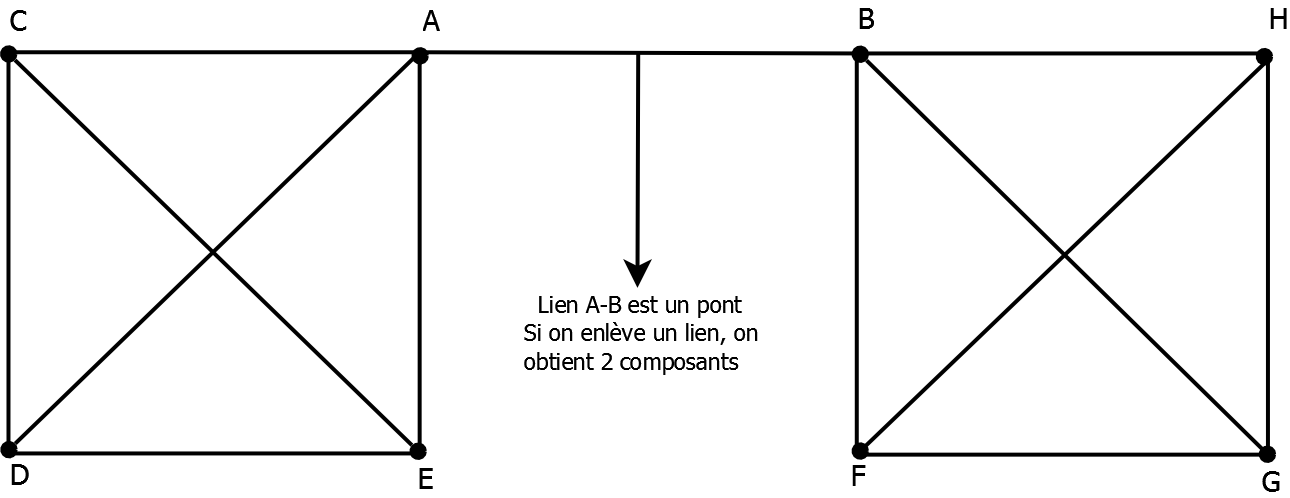
\includegraphics[scale=0.4]{images/18_Pont.png}
    \caption{\label{Pont} Pont}
    \end{figure}
    
    \begin{figure}
    \center
    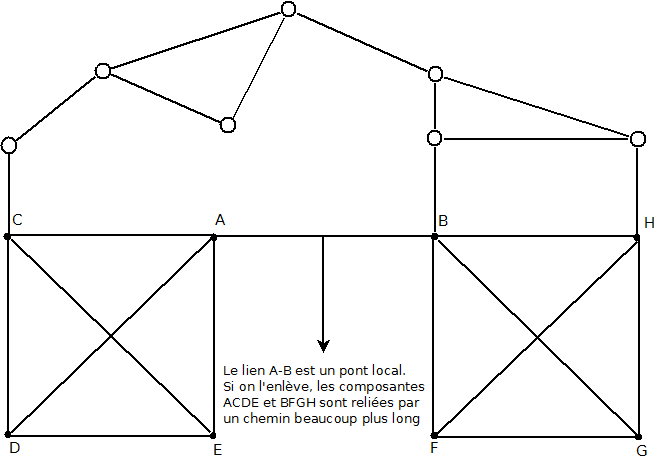
\includegraphics[scale=0.5]{images/18_Pontlocal.png}
    \caption{\label{Pontlocal} Pont local}
    \end{figure}